%REACTION TIME AND FALLING BODIES
\newexp
{\bf Note:} We will not be doing this experiment this year.
Nevertheless, no special equipment is required and you are encouraged
to try this lab on your own.

\begin{tabbing}
reference12345 \= col2 \kill
References: \> {\em An Introduction to Error Analysis}, John R.\ Taylor,
   chapters 4, 5.  We strongly \\
\> recommend this book for students majoring in pre-engineering or
the physical \\
\> sciences. \\
\end{tabbing}

\section*{Before Lab}
This experiment relies heavily on the material developed in Appendix A
of this lab manual---Please review it carefully.  And of course, study
this writeup carefully.

\section*{Introduction}
     In this experiment we will measure the reaction times of the
experimenters as a way of examining the random scatter in
experimental data.  We will also introduce the {\em standard deviation}
 as a measure of
that scatter.  Keep in mind that experimental scientists
distinguish between random error and systematic error; we will be
concerned only with the former in this experiment.  See Taylor
and Appendix A in the lab manual (p.~\pageref{scierror})
for a more complete discussion.

\section*{Analysis of Problem}
      One normally thinks of measuring a given physical
quantity with a particular instrument.  For example, one
ordinarily measures length or distance with a meter stick, time
with a clock, mass with a balance, and so on.  In this exercise,
however, we will see how one can measure reaction time with a
meter stick.  We will also study the random variations in the
data and the way one can estimate the ``best" value of the
reaction time.

We can find a person's reaction time by measuring the distance fallen
by a meterstick and using the law of falling bodies to calculate the
time it has taken to fall that distance.  If we let $D$ represent the
distance, $t$ the time, and $g$ the acceleration of gravity, then
\begin{equation}
D = {{1} \over {2}} \: g t^{2}  \label{eq:react1}
\end{equation}
We will solve this equation for time to find time as a function
of distance fallen.

\section*{Experimental Procedure}
     Two people working together can measure their reaction times
as follows:  One person holds a meter stick by its upper end.
The second person, whose reaction time is to be measured, places
one or both hands lower on the stick, in a position that can be
reproduced from one measurement to the next.  Without warning,
the first person drops the stick.  The second person closes his
or her hand so as to grab the stick.  Then s/he records the
distance the stick fell. This procedure should be repeated 40
times, maintaining the experimental conditions as nearly alike as
possible for all the measurements.  {\bf PLEASE NOTE:}  You should work
out your procedure carefully and describe it {\em in detail} in your
laboratory notebook before you take your measurements.  For
example, how did you make sure your hand didn't move up or down
as you grabbed the meter stick?  What other potential problems
did you consider?   And so on---be complete in describing your procedure.

     In formulating your procedure, you should also consider how
accurate your measurements will be, and what steps you might make
to improve that accuracy.  Even though these will not be
measurements of high precision, you should be able to measure
each distance to better than one centimeter.  However, one can
hardly expect to be as accurate as
one millimeter, at least without much fancier apparatus.
You should also estimate how accurate your times
will be, given the accuracy with which you can measure distance.

\section*{Reduction and Analysis of Data}
     Note that, even with care, successive measurements will not
give exactly the same result. This situation arises in making and
analyzing measurements of all sorts and will be the focus of our
analysis in this experiment.

     We must begin by converting all our distances into reaction
times, using Equation~\ref{eq:react1}.  (Note that we cannot find the average
reaction time simply by averaging the distances and converting
the average distance into an average time, since the average of
the squares of a series of numbers is not equal to the square of their
average.  Note for example that for the two numbers 3 and 5, the
average of their squares, 17, is not the same as the square of
their average, 16.  This example shows that one needs to convert
all of the measured distances into the corresponding times.)

     The conversion from the measured distances to the
corresponding times can be calculated using Equation~\ref{eq:react1}.
One can use a calculator, but you may also use a spreadsheet such as
the one in Linfit to do these calculations if you prefer.

     Record your calculated reaction times and your estimate of
their uncertainties in a data table.  You are now ready to start
the data analysis.

     When an experimental quantity --- time, in this case --- is
measured several times the results obtained are often influenced
by a number of factors that fluctuate in an independent and random
fashion.
(What are some of those factors in this experiment?)  Some of the
factors may make the measurement appear larger and some smaller.
Usually, most of the measurements will lie near
the center of the observed range rather than be very large or
very small compared with the average.  To learn very much from a
series of measurements of a quantity, one needs to decide what is
the ``best" value of the quantity and also to obtain a number
which describes the range of variation on either side of the
``best" value.

     If the experimental conditions do not change during a series of
measurements, the ``best" value of the result is usually the
average or mean.  To obtain your average reaction time, add
together the individual times and divide by the total number:
\begin{equation}
\mbox{average time} = A = {{(t_{1} + t_{2} + \cdots + t_{N})} \over {N}}
   \label{eq:react2}
\end{equation}
where $A$ is the average time and $N$ is the number of measurements.

     To describe the data more completely, one
needs to specify the range or spread that characterized the data.  One
might simply specify the lowest and highest values observed; but this
procedure is often misleading because very often one point will
be much higher or much lower than any other.  A more common way
of describing the spread of results is to give a number which,
when added to or subtracted from the average result, will give
values which include about 2/3 of all the measurements.  This
number describing the spread of results is called the {\em standard
deviation} of the measurement and is usually designated by $\sigma$
(the lower case Greek letter sigma.

\paragraph*{Determination of Standard Deviation from Experimental Data}

     We begin with the definition of the deviation.  For the $i$th
data point, the deviation $d_{i}$ is defined as
\begin{equation}
d_{i} = t_{i} - A  \label{eq:react3}
\end{equation}
Intuitively, the sum of the absolute value of deviations divided by the number of
measurements  should provide a reasonable
measure of the scatter in the data.  This quantity is called the
average deviation---see Appendix A.

However,
a more rigorous and widely used measure
turns out to be the standard deviation $\sigma$, defined as
\begin{equation}
\sigma = \sqrt { {{1} \over {N - 1}} \: \sum_{i} \, d_{i}^{2} }
  \label{eq:react4}
\end{equation}
It can be shown that under most circumstances, about 2/3 of the
observations should lie within one standard deviation of the
average value.

     We will employ a graphical procedure to investigate this
claim.  First, along a line, lay out a scale that will cover the
range of measurements in the whole group.  Then make a mark on
the scale to represent each one of the measurements, as shown in
Fig.~\ref{fig:react1}.  If two or more of the measurements result in exactly
the same value, make one mark above the other so both can be recorded
as being on that point of the line.  Next, determine the average
value of all the measurements and mark that point on the line as
point $A$.  Count the number of points along the line that
correspond to values of the measurement smaller than $A$ and mark
the point ($A - \sigma$) which divides this group so that about 2/3 of the
points below $A$ are are between $A$ and ($A - \sigma$).
\begin{figure}
\begin{center}
{\resizebox{5.1in}{!}{{\includegraphics{reactionC.eps}}}}
\end{center}
%\vspace{0.75in}
% \centerbmp{5.1in}{.86in}{reaction.bmp}
 \caption{Sample distribution diagram of reaction time data.   \label{fig:react1}}
\end{figure}
Mark the point ($A + \sigma$) which divides the points above $A$ so that
about 2/3 of them are between $A$ and ($A + \sigma$).

     If the distribution of points about the average value is
symmetric, the distance along the scale from $A$ to ($A - \sigma$) will
equal the distance along the scale from $A$ to ($A + \sigma$), and this
distance $\sigma$ will be the standard deviation of this set of
measurements.  Thus we can say that about two measurements in
three will lie in the range ($A \pm \sigma$).

     If the distance from $A$ to ($A - \sigma$) is slightly different from
the distance from $A$ to ($A + \sigma$), one can obtain an approximate value
for the standard deviation by taking half the distance from ($A - \sigma$)
to ($A + \sigma$).  If these two distances are greatly different, the
concept of standard deviation may not applicable to the set of
data.  In this asymmetric case one should give the spreads of the
data in both the upward and the downward direction which include
2/3 of the points on either side in the form
\[
A^{+U}_{-L}
\]
     Still a third indication of the spread of a set of data is
called the ``probable error", which includes one half of all the
measurements within its limits.  When writing a result as ($A \pm B$)
one should identify which measure of the spread is being used.
The standard deviation, which is easily calculated on a computer
and on many pocket calculators, is the most commonly used
measure.

\paragraph*{Normal Distribution of Errors}

     To aid one in understanding the fluctuations in the results
of a measurement it is often helpful to draw a bar-graph or
histogram similar to the one shown in Fig.~\ref{fig:react2}.  In drawing this
graph one needs to divide the points plotted in Fig.~\ref{fig:react1} into
groups which are broad enough to smooth out the major
fluctuations but are not so wide as to mask the general trends.
\begin{figure}
\begin{center}
{\resizebox{5in}{!}{\rotatebox{-90}{\includegraphics{fig3.2.ps}}}}
\end{center}
% \vspace{3.25in}
% \hspace{.5in}
% \special{bmp:bgphnorm.bmp x=4.79in y=3.25in}
\caption{Bar graph (normal distribution).  \label{fig:react2}}
\end{figure}
\begin{figure}
\begin{center}
{\resizebox{5in}{!}{\rotatebox{-90}{\includegraphics{fig3.3.ps}}}}
\end{center}
% \vspace{2in}
% \hspace{1in}
% \special{bmp:bgphnon.bmp x=4.12in y=2in}
 \caption{Bar graph (non-normal distribution).  \label{fig:react3}}
\end{figure}
     In an ideal or normal distribution of random errors this
graph has one peak and is symmetric about the average value.  In
some situations, where there is an unexpected change in the
quantity being measured, there may be two peaks, as shown in
Fig.~\ref{fig:react3}.  In the other cases the distribution will extend much
further on one side of the average than on the other.  In case of
such non-normal distributions one should not try to represent the
results by a single average and standard deviation.

\paragraph*{Standard Deviation of the Mean}

     The standard deviation is a measure of the average
uncertainty of {\em an individual data point} --- that is, if we know the
standard deviation $\sigma$ and the average $A$, we know that the chances
are about 2 in 3 that any {\em single} point will lie in the range
$A \pm \sigma$.

But it is reasonable to suppose that our knowledge of
the average value is more accurate (or less uncertain)
than our knowledge of any single data point.
     Indeed, this statement can be shown to be correct.  The
appropriate uncertainty in the {\em average value} of a set of
measurements is the {\em standard deviation of the mean}, defined as
\begin{equation}
S = {{\sigma} \over {\sqrt{N}}}  \label{eq:react5}
\end{equation}
where $N$ is the number of data points used in determining $\sigma$.

     If one takes more data points for a given measurement, the
spread in those points, described by $\sigma$,  probably will not
change much, but the accuracy of their average, described by $S$,
will improve as $N$ becomes larger.  {\bf PLEASE NOTE:}  In reporting a
measurement, always state explicitly whether you are citing a
standard deviation or a standard deviation of the mean.

Please see Appendix A for a more complete discussion.

\paragraph*{Analyzing your Reaction Time Data}

\begin{enumerate}
\item Divide your data into two groups, using the first 20 points as
   one group and the second 20 points as the other.
\item For each group separately make a data distribution diagram as
   shown in Fig.~\ref{fig:react1}.
\item Calculate the average value for each group, $A_{1}$ and $A_{2}$, and
   mark $A_{1}$ and $A_{2}$ on its diagram.
\item For each group mark on the diagram the points ($A + \sigma$) and
 ($A - \sigma$).
   Using the 2/3 criterion, determine the standard  deviations for
   each group and compare them with the values obtained using
   Equation~\ref{eq:react4}.  You may find it convenient to use
   a spreadsheet for these calculations.
%
\item Using Equation~\ref{eq:react5}, compute the Standard Deviation of the Mean
for each group.
\item Compare the results of your group 1 with the results of group 2.
   One can say the results are highly consistent if the absolute value of the
   difference
   between $A_{1}$ and $A_{2}$ is less than ($S_{1} + S_{2}$).
If $|A_{1} - A_{2}|$ is
   less than 2($S_{1} + S_{2}$), the results are moderately consistent.
   If $|A_{1} - A_{2}|$ is more than 2($S_{1} + S_{2}$), there may have been a
   trend in your response as you gained experience in grabbing the
   meter stick, or perhaps some other source of systematic error is present.
\item Compute $A$, $\sigma$, and $S$ for the whole set of data and compare your
    results with those of others in your class.  For this part use
    Equations~\ref{eq:react4}~and~\ref{eq:react5}.
%
\item Draw a distribution bar graph as shown in Fig.~\ref{fig:react2} for the
    whole set of data.  How well does it resemble a ``Normal" distribution?
\end{enumerate}

\section*{Conclusions}
Make a careful table listing all your numerical results and their
uncertainties, and give a careful discussion of them.
Comment on the consistency of your results and how they compare to the
results of others in your class.  Mention any sources of error, both
systematic and random.

\section*{Critique of Lab}
     Follow the suggestions given in the Introduction to the
Laboratory Manual.

